\documentclass[tikz,border=6pt]{standalone}
\usepackage[T1]{fontenc}
\usepackage[utf8]{inputenc}
\usepackage{pgfplots}
\usepgfplotslibrary{groupplots}
\usetikzlibrary{calc}
\pgfplotsset{compat=1.18}
\begin{document}
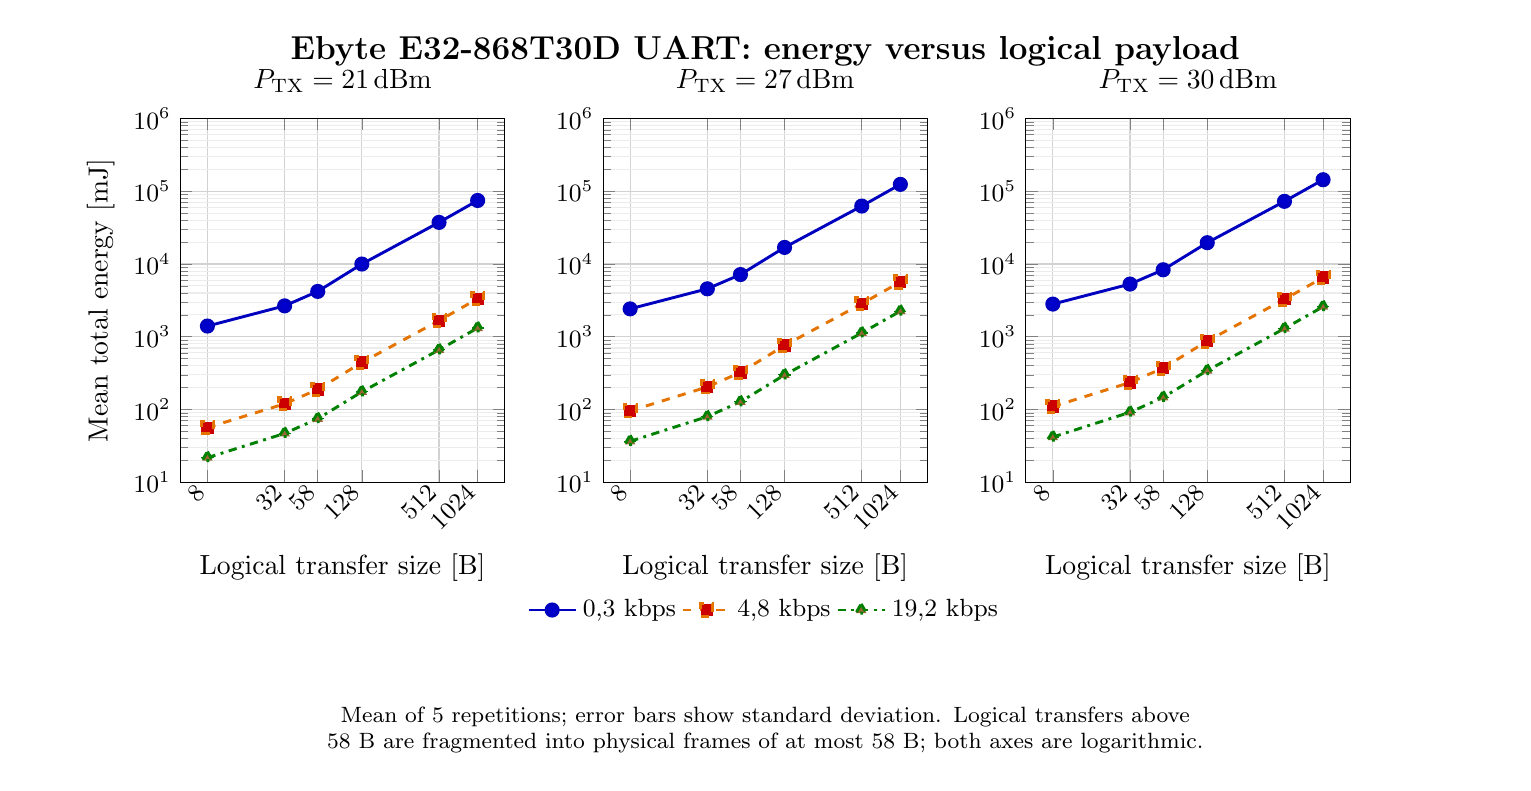
\begin{tikzpicture}
\begin{groupplot}[/pgf/number format/use comma,
  group style={group size=3 by 1, horizontal sep=1.25cm},
  width=5.7cm, height=6.2cm,
  xmode=log, log basis x={2}, ymode=log, log basis y={10},
  ymin=10, ymax=1000000,
  xtick={8,32,58,128,512,1024}, xticklabels={8,32,58,128,512,1024},
  x tick label style={rotate=45, anchor=east, font=\small},
  y tick label style={font=\small},
  grid=both, minor grid style={gray!15}, major grid style={gray!35},
  xlabel={Logical transfer size [B]},
  every axis plot/.append style={line width=1.05pt},
  error bars/error bar style={line width=0.35pt},
  legend style={font=\small, draw=none, fill=none, at={(0.5,-0.29)},
    anchor=north, legend columns=-1},
]
\nextgroupplot[title={\(P_{\mathrm{TX}}=21\,\mathrm{dBm}\)}, ylabel={Mean total energy [mJ]}]
\addplot+[
  color=blue!75!black, solid, mark=*, mark size=2.2pt,
  error bars/.cd, y dir=both, y explicit,
] coordinates {
  (8,1403.35259) +- (0,0.843571759)
  (32,2660.54034) +- (0,1.03305967)
  (58,4202.79178) +- (0,1.61195132)
  (128,9998.55866) +- (0,5.9089365)
  (512,37387.4384) +- (0,44.9452002)
  (1024,74806.3696) +- (0,100.395047)
};
\addplot+[
  color=orange!90!black, dashed, mark=square*, mark size=2.2pt,
  error bars/.cd, y dir=both, y explicit,
] coordinates {
  (8,56.3154406) +- (0,0.0862633137)
  (32,119.592625) +- (0,0.160962083)
  (58,188.590801) +- (0,0.208408123)
  (128,443.396512) +- (0,0.687524417)
  (512,1666.96349) +- (0,0.599978602)
  (1024,3333.73678) +- (0,0.721469965)
};
\addplot+[
  color=green!50!black, dashdotted, mark=triangle*, mark size=2.2pt,
  error bars/.cd, y dir=both, y explicit,
] coordinates {
  (8,21.7680975) +- (0,0.0287147447)
  (32,46.8926026) +- (0,0.0375599895)
  (58,74.6625213) +- (0,0.0726162245)
  (128,174.945831) +- (0,0.245758162)
  (512,660.753558) +- (0,0.658958528)
  (1024,1320.718) +- (0,0.374417393)
};
\nextgroupplot[title={\(P_{\mathrm{TX}}=27\,\mathrm{dBm}\)}]
\addplot+[
  color=blue!75!black, solid, mark=*, mark size=2.2pt,
  error bars/.cd, y dir=both, y explicit,
] coordinates {
  (8,2420.06446) +- (0,2.53149896)
  (32,4565.52523) +- (0,5.56802645)
  (58,7169.26858) +- (0,7.65035462)
  (128,16920.7517) +- (0,17.1921011)
  (512,62673.1727) +- (0,38.3243947)
  (1024,124598.102) +- (0,242.404941)
};
\addlegendentry{0{,}3 kbps}
\addplot+[
  color=orange!90!black, dashed, mark=square*, mark size=2.2pt,
  error bars/.cd, y dir=both, y explicit,
] coordinates {
  (8,95.53469) +- (0,0.0737074672)
  (32,204.446184) +- (0,0.242406155)
  (58,322.642142) +- (0,0.28521904)
  (128,758.78457) +- (0,0.596833398)
  (512,2845.43414) +- (0,3.49833507)
  (1024,5668.94352) +- (0,8.72246097)
};
\addlegendentry{4{,}8 kbps}
\addplot+[
  color=green!50!black, dashdotted, mark=triangle*, mark size=2.2pt,
  error bars/.cd, y dir=both, y explicit,
] coordinates {
  (8,36.4998202) +- (0,0.0214172299)
  (32,79.8270292) +- (0,0.0454415299)
  (58,127.705287) +- (0,0.1219832)
  (128,298.701639) +- (0,0.311634982)
  (512,1128.34058) +- (0,1.48063483)
  (1024,2251.7146) +- (0,1.52912638)
};
\addlegendentry{19{,}2 kbps}
\nextgroupplot[title={\(P_{\mathrm{TX}}=30\,\mathrm{dBm}\)}]
\addplot+[
  color=blue!75!black, solid, mark=*, mark size=2.2pt,
  error bars/.cd, y dir=both, y explicit,
] coordinates {
  (8,2814.28226) +- (0,4.13387105)
  (32,5305.48879) +- (0,4.70177109)
  (58,8339.70933) +- (0,10.3552026)
  (128,19664.3831) +- (0,14.0746809)
  (512,72822.727) +- (0,39.2063401)
  (1024,144285.274) +- (0,439.556555)
};
\addplot+[
  color=orange!90!black, dashed, mark=square*, mark size=2.2pt,
  error bars/.cd, y dir=both, y explicit,
] coordinates {
  (8,109.657169) +- (0,0.0590503996)
  (32,235.08446) +- (0,0.204491425)
  (58,371.226943) +- (0,0.189004648)
  (128,872.800056) +- (0,0.814247858)
  (512,3275.17529) +- (0,3.78936838)
  (1024,6525.03387) +- (0,11.3160782)
};
\addplot+[
  color=green!50!black, dashdotted, mark=triangle*, mark size=2.2pt,
  error bars/.cd, y dir=both, y explicit,
] coordinates {
  (8,41.748603) +- (0,0.0361675683)
  (32,91.6482983) +- (0,0.033292413)
  (58,146.891371) +- (0,0.0511492973)
  (128,343.362814) +- (0,0.269087228)
  (512,1298.43098) +- (0,1.86862391)
  (1024,2590.62142) +- (0,2.57680654)
};
\end{groupplot}
\node[font=\bfseries\large] at ($(group c2r1.north)+(0,0.85cm)$)
  {Ebyte E32-868T30D UART: energy versus logical payload};
\node[font=\footnotesize, align=center, text width=18.5cm]
  at ($(group c2r1.south)+(0,-3.15cm)$)
  {Mean of 5 repetitions; error bars show standard deviation. Logical transfers above 58 B are fragmented into physical frames of at most 58 B; both axes are logarithmic.};
\end{tikzpicture}
\end{document}
